\section{Fundamentação teórica}
Lorem ipsum dolor sit amet, consectetur adipiscing elit. Nam sapien libero, fermentum ac sapien id, iaculis pellentesque justo. Vestibulum congue turpis nisi, ac posuere justo feugiat ultrices. Fusce eu ipsum risus. Nam molestie volutpat lacus quis consequat. Proin facilisis urna non sem luctus, sit amet laoreet arcu dictum. Cras porttitor molestie gravida. Integer vulputate at dui nec egestas. Mauris diam quam, sodales et ipsum in, efficitur pretium eros. Phasellus vestibulum quam nibh, vestibulum elementum magna porta id. Phasellus enim quam, aliquet accumsan nunc nec, porttitor ultrices augue. Aenean semper sapien sit amet dolor consectetur, eu sagittis dui vestibulum. Pellentesque nec mollis ex. Donec vitae commodo urna, gravida rutrum mauris. Mauris egestas nisl a felis pharetra, ac tincidunt eros facilisis. Vestibulum faucibus bibendum consectetur. Nunc sit amet magna suscipit, suscipit urna in, auctor nunc \ref{figura1}.

Aenean sit amet nulla sem. Integer venenatis, eros eget fermentum aliquam, nibh massa mattis elit, eu tincidunt odio nulla sit amet velit \cite{knuth:84}. Nulla lobortis sit amet mi vel suscipit. Cras tristique rhoncus mi a ultrices. Vestibulum mi eros, placerat at finibus vitae, elementum id tellus. Aenean sit amet ex id odio cursus sodales. Sed placerat et mi et porta. Morbi massa lacus, consequat quis scelerisque in, blandit nec eros. In aliquet felis ut faucibus laoreet. Phasellus luctus consectetur enim, quis ornare dui pulvinar id \ref{tabela1}.

\begin{figure}
\centering
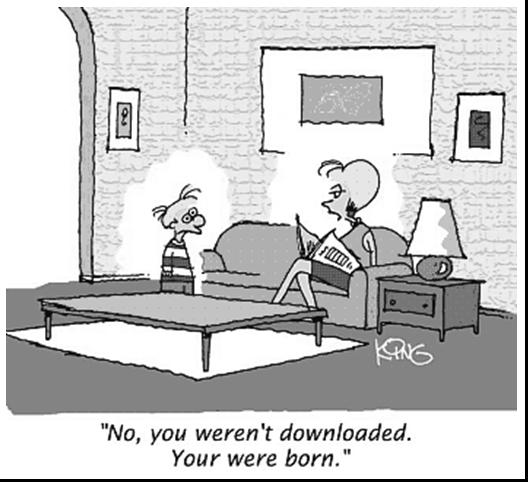
\includegraphics[width=.5\textwidth]{secoes/figuras/fig1.jpg}
\caption{A legenda das figuras devem ser posicionadas na parte inferior.}
\label{figura1}
\end{figure}